\chapter{Proposed Method}
\label{proposed}
\thispagestyle{empty}

\begin{quotation}
{\footnotesize
\noindent{\emph{``Summer: A city of Grandpas? \\
Morty: It's the Citadel of Ricks. All the different Ricks from all the different realities got together to hide here from the government. \\
Summer: But if every Rick hates the government, why would they hate Grandpa? \\
Morty: Because Ricks hate themselves the most. And our Rick is the most himself.''}}
\begin{flushright}
Rick and Morty (Season 3, Episode 1)
\end{flushright}
}
\end{quotation}



\vspace{0.5cm}

In control theory, hierarchical architectures, where several layers of control interact, are extensively used. A very simple example is the cascaded control structure designed for a DC Motor where the outer loop (high level, slower) ensures that the actual speed is always equal to reference speed. In order to achieve its goal the outer loop outputs a reference torque/current which is received by the inner loop (low level, faster) that controls the torque via armature current and keeps the current in a safe limit. 

The design tool of control theory to approach hierarchical schemes is the block diagram. It gives the intuition of layered loops and cascaded structures. Block diagrams are much in use in control theory since they are often more convenient devices to analyze or design a system than the transfer function of the overall system. They are basically a composition of modular subsystems. These subsystems are represented as blocks that include the transfer function of the corresponding subsystem. The interconnections among subsystems are represented with directed lines illustrating the signal flow. We introduce these objects to hierarchical reinforcement learning with small differences that are necessary in the context of learning. The goal is to obtain a generic framework for the design of the hierarchy in reinforcement learning. This framework is a computational graph that contains various types of blocks referring to subsystems. Unlike the block diagram of control theory, in our approach blocks and the interconnections are of various nature.

In our scheme one cycle of the computational graph corresponds to a step in the environment. At each step, environment observation is retrieved in the form of a reward and a state data. A state can be absorbing or not. If it is, then the graph is at the last cycle of the current episode. Otherwise, an action, taken from the last block in the graph, is applied and the environment state is observed once again and so on. Data flow in the graph through connections between blocks. There are three types of connections: input, reward, and alarm connections. Input connections correspond to the connections in the conventional block diagram. They transport input and output data between blocks. We call the input signal of a block as \textit{state} and the output as \textit{action}. It should be remarked that the terms state and action here do not refer to the content of the data carried but to the manner in which the receiving block perceives them. For instance, reward data of the environment can be observed as the state by some blocks. Hence, the connection that carries the reward would be the input connection.

RL agent aims to approximate an optimal behavioral strategy while interacting with its environment. It evaluates its behavioral strategy based on an objective function $(\mathcal{J})$ that is computed with rewards. These rewards can be extrinsic or intrinsic. Extrinsic rewards are in the formalization of the environment. They are retrieved through observation. Intrinsic rewards can be constructed by the designer using the state information. In optimal control, typically, the performance indicator is the cost function $(\mathcal{C = -J})$ and the optimal control goal is to find a control law that minimizes the cost function. In optimal control, the cost function is optimized at design time. That is, unlike the RL agent, during its operation, the controller does not need a metric to evaluate and update its behavior. This contrast reflects in our framework into another type of connection that carries only the reward information. An explicit reward connection definition is needed. Reward connection implies that the data carried will be used as a performance metric and not as an input to the block. 

In hierarchical approaches to RL, typically, high level agents do not take actions at each step. To enforce this structure in our framework, blocks that are in the higher levels of the hierarchy are not activated in some cycles. Their output remains unchanged for those time steps. Once the lower level blocks complete their episode they activate the upper level ones by sending a signal trough alarm connections. 

\begin{figure}[t]
      \centering
      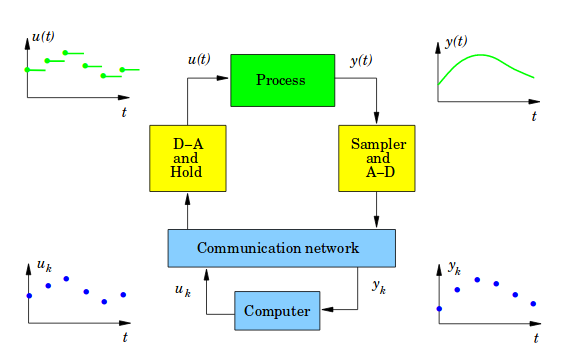
\includegraphics[width = \textwidth]{./pictures/digitalcontrol.png}
      \caption[Digital control system]{Schematic of a digital control system}
      \label{fig:digitalcontrol}
\end{figure}

In this scheme, alarms are analogous to events in event-based control systems. Event-based control systems are digital control methods. Figure~\ref{fig:digitalcontrol} shows a typical architecture for a digital controller. The process is a continuous-time physical system to be controlled. The input and the output of the process are continuous-time signals. Thus, the output needs to be converted and quantized in time before being sent to the control algorithm. This process is called \textit{sampling}. There are two ways of designing digital controllers: periodic and event-based trigger. The traditional way to design digital control systems is to sample the signals equidistant in time, that is, periodically~\cite{aastrom1997computer}, using a clock signal.  

Event based sampling is an alternative to periodic sampling. Signals are sampled only when significant events occur. This way, control signal is applied only when it is required, so as to better cope with various constraints or bottlenecks in the system. A block diagram of a system with event based control is shown in \ref{fig:eventbased}. 

\begin{figure}[t]
	\centering
    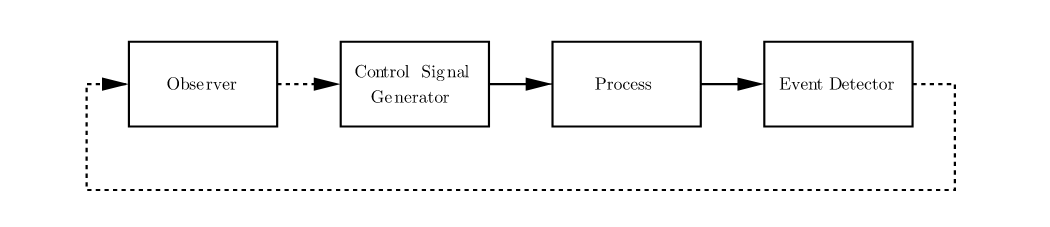
\includegraphics[width=\textwidth]{./pictures/eventbased.png}
    \caption[event-based control]{Block diagram of a system with event-based control. Solid lines denotes continuous signal transmission and the dashed lines denotes event based signal transmission}
    \label{fig:eventbased}
\end{figure}
  
The system consists of the process, an event detector, an observer, and a control signal generator. The event detector generates a signal when an event occurs, typically when a signal passes a level, possibly with different events for up-and down-crossings. The observer updates the estimates when an event occurs and passes information to the control signal generator which generates the input signal to the process. The observer and the control signal generator run open loop between the events. The dashed lines of Figure~\ref{fig:eventbased} correspond to the alarm connections in our framework. In HRL approaches, typically a lower-level algorithm returns to the higher-level one once it has completed its subtask. It can be due to an absorbing state terminating either with success or failure, or simply a horizon reach. The event of event-based control thus corresponds to the end of a subtask of a low-level agent in HRL. 

In control theory, each block of the block diagram refers to a subsystem such as a plant, a controller or a sensor, and contains the corresponding transfer function or state-space equation matrices. Either way, it includes an expression of how the incoming signal is manipulated. \ref{fig:blockdiagramofcontrolth} depicts an example structure. Apart from the blocks and connections, there are circle shaped objects in the diagram which represent basic arithmetic operations applied to the incoming signals. 

\begin{figure}[t]
      \centering
      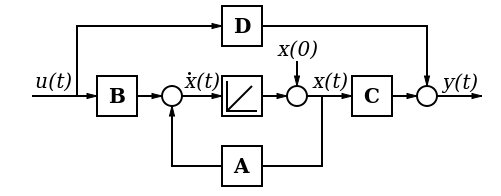
\includegraphics[width = 0.8\textwidth]{pictures/blockdiagramofcontrolth.png}
      \caption{Example of a conventional block diagram}
      \label{fig:blockdiagramofcontrolth}
\end{figure}

Blocks in our framework have subtle differences. The manner in which the signal is manipulated explicitly depends on the type of the block. The input-output relation of some of the blocks have a discrete-time dynamic behavior. They keep track of the state and store information. That is, they are stateful and their operation can be described with a discrete-time transfer function. \textit{function block} is the most similar kind to a conventional block of control theory. Its operation on the incoming signal is deterministic. In other words, it has a deterministic policy chosen by the designer of the system. Function block is an example to stateless blocks. A type of function block performs simple arithmetic operations on the incoming signals. They are named as \textit{basic operation blocks}. 

Control block is the learning part of the system. It is associated to a policy and a learning algorithm. It calls the policy to take an action and uses the learning algorithm to update the policy. This learning algorithm can be policy search-based (e.g. GPOMDP, PoWER) or value-based (e.g. Q-learning, SARSA($\lambda$)) and the policy can be a parameterized one (e.g. Gaussian) or a Q-value-based one (e.g. Boltzmann, $\epsilon$-greedy). Control blocks accumulate each trajectory sample in a dataset. Once the policy is to be updated, this dataset is passed to the learning algorithm. Similarly to the MDPs a sample $\left\langle s,a,r,s'\right\rangle$ consist of state, reward, action and next state data, being the input, the output and the reward of the block.
In a control block the state and reward data are manipulated separately. State data flow is used for computing the value of the blocks and action, i.e. running the system, whereas the reward data flow is the flow of the evaluation of the performance. Thus, control block needs reward connections to be isolated from the input connections.

Naturally, control blocks are the only blocks at the receiving ends of the reward connections as they are the only learning members. The other blocks may also take extrinsic reward data from the environment. However, they will not perceive it as a performance metric. Thus, they will receive the data through input connections instead of a reward connection.

If the control block is in a lower level of the hierarchy, it can signal the end of its episode to the higher level blocks. The end of an episode can be reached due to an absorbing state with failure or success or a horizon reach. The control block that is in the higher levels of the hierarchy does not take an action until it receives an alarm signal or an indicator of a last step of the environment.  

Apart from the end of an episode of a control block, custom events can be created to produce alarm signals. Event blocks are used with this objective. 
They have custom methods with binary results.

Since some of the control blocks are \textit{awake} only at certain times, some measures needs to be taken to protect the integrity of their dataset. Reward data coming from the environment must not be lost when the high level control is inactive. Reward accumulator block accumulates the input reward until the alarm is up. With the alarm, accumulated data is passed to the controller and the accumulator is emptied. Obviously, the alarm source that is connected to a high level controller needs to be the same as the one that is connected to the reward accumulator that passes its data to that controller. Since the reward accumulator stores information, it is an example of a stateful block.

Another example of a stateful block is the error accumulator. Error accumulator block accumulates the incoming error data and passes it at each step to a control block. When one of its alarms activates or the environment state is the last of the episode it resets the accumulator to zero. Integration in discrete time corresponds to accumulation. The control block that has an error accumulator as an input connection applies integral action. 
  
Placeholders operate as the representation layer of the environment. In the conventional block diagram, the model of the plant is a part of the block diagram. Typically, it receives control signal as an input and outputs the state data to the rest of the blocks. It contains the transfer function of the plant model. In our framework, the model itself is not a part of the diagram. This is primarily because we focus on model-free learning, thus we do not have a mathematical expression of how the environment reacts to inputs, nor its estimation. The only information we have comes from the step samples. The other reason is that blocks may need to observe different parts of the environment. For instance, a block may require only the reward to operate whereas the other one may need both the state and the reward. Such isolation of observation data is achieved with placeholders. At each cycle of the graph, state and the reward output of the environment are passed through the related placeholders, the state and reward placeholders. In addition, last action applied to the environment is also saved in a placeholder called last action placeholder. These blocks do not operate on or manipulate the data they receive. Instead, they function as a bridge or a network between the environment and the diagram. 

Selector blocks implement the mode switching behavior in our framework. They contain block lists and activate one list at each cycle. The selection is done according to the first input of the selector block. Once a list inside the selector block is activated all the other inputs to the selector block are passed to the first block of the selected list. The reward and alarm connections of the blocks inside the selector block are independent from the selector. That is, selector block does not have reward connections and its alarm connections are not passed to the blocks in the block lists. Selector block strengthens the flexibility of our framework for hierarchical schemes by allowing hybrid schemes to join the picture. Higher level controller applies an action depending on the state and this action activates an underlying behavior provided by the selected block list in the selector block.


